\chapter{The Drupal structure}

\section{Structural elements}

Drupal 8 core defines eight types of structural elements. To see an overview of these elements click on the \textbf{Structure} button in the administrative menu (Figure \ref{fig:structural_elements}).

  \begin{figure}[H]
  	\centering
  	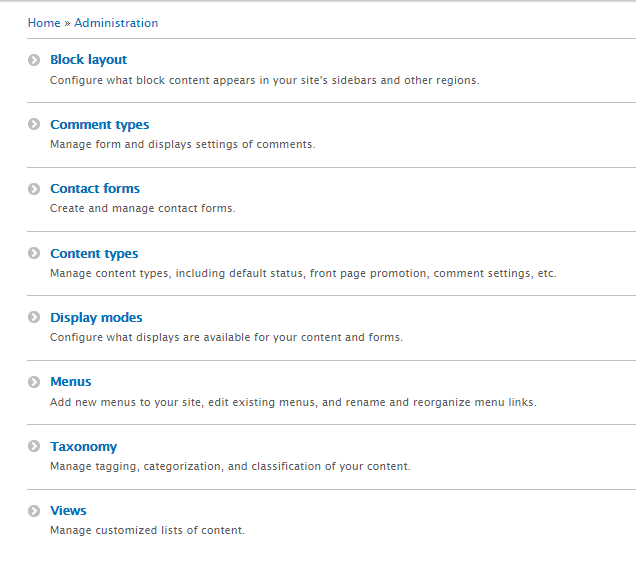
\includegraphics[width=\textwidth]{chapter4/structural_elements}
  	\caption{Structural Elements}
  	\label{fig:structural_elements}
  \end{figure} 
  
  Each of these elements has a certain use within Drupal. The following list describes each of the structural elements. Don't worry if not all the elements are clear to you, when you start changing and using your site the structure will become clear.
  
  \begin{description}
  	\item[Block layout:] Blocks are site elements which can be positioned in different places on your site. For example the search field, which is visible on the left side of your first Drupal page, is a Drupal block. You can put a block in different places on your page, these places are called \textbf{regions}. These regions depend on the Drupal theme you are using. 
  	When you click the \textbf{Block layout} link you will see the following page (Figure \ref{fig:block_layout}).
  	
  	\begin{figure}[H]
  		\centering
  		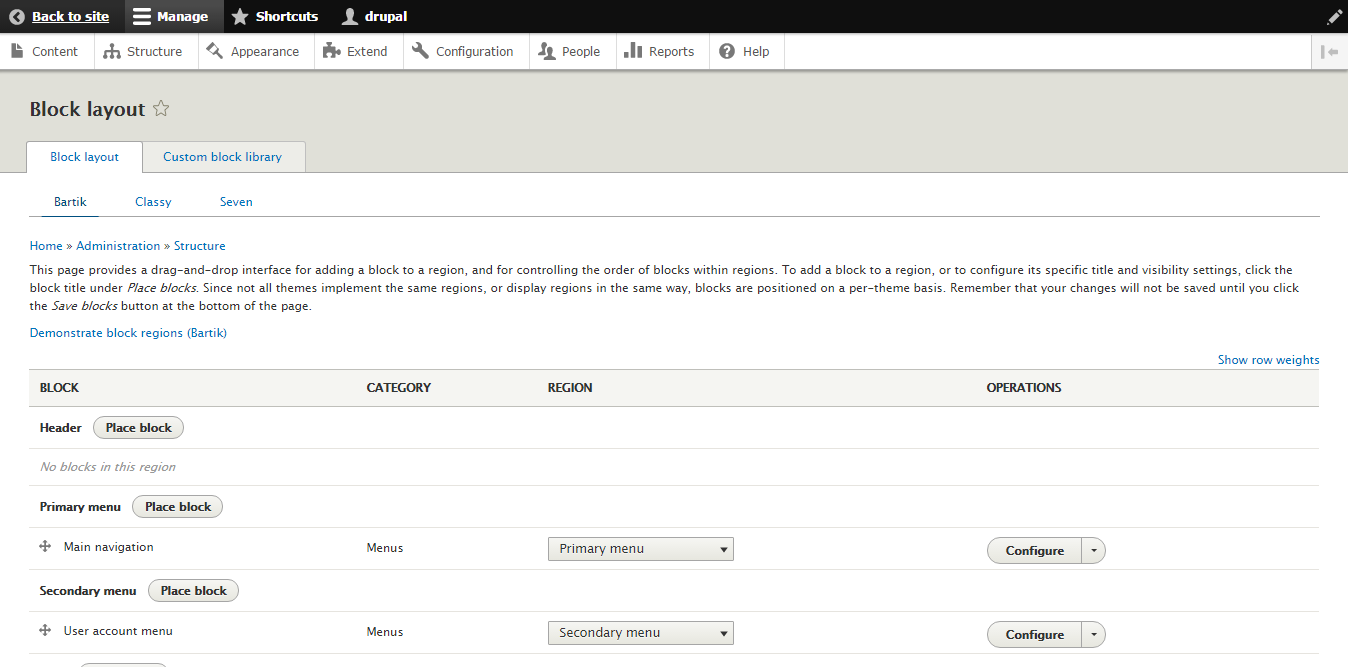
\includegraphics[width=\textwidth]{chapter4/block_layout}
  		\caption{Block layout}
  		\label{fig:block_layout}
  	\end{figure} 
  	
  	This page shows a list of the different regions and allows you to add blocks to each of these regions. You can click the link \textbf{Demonstrate block regions(Bartik)} to view the regions of the current theme (Bartik) (Figure \ref{fig:region_demo}).
  	
  	\begin{figure}[H]
  		\centering
  		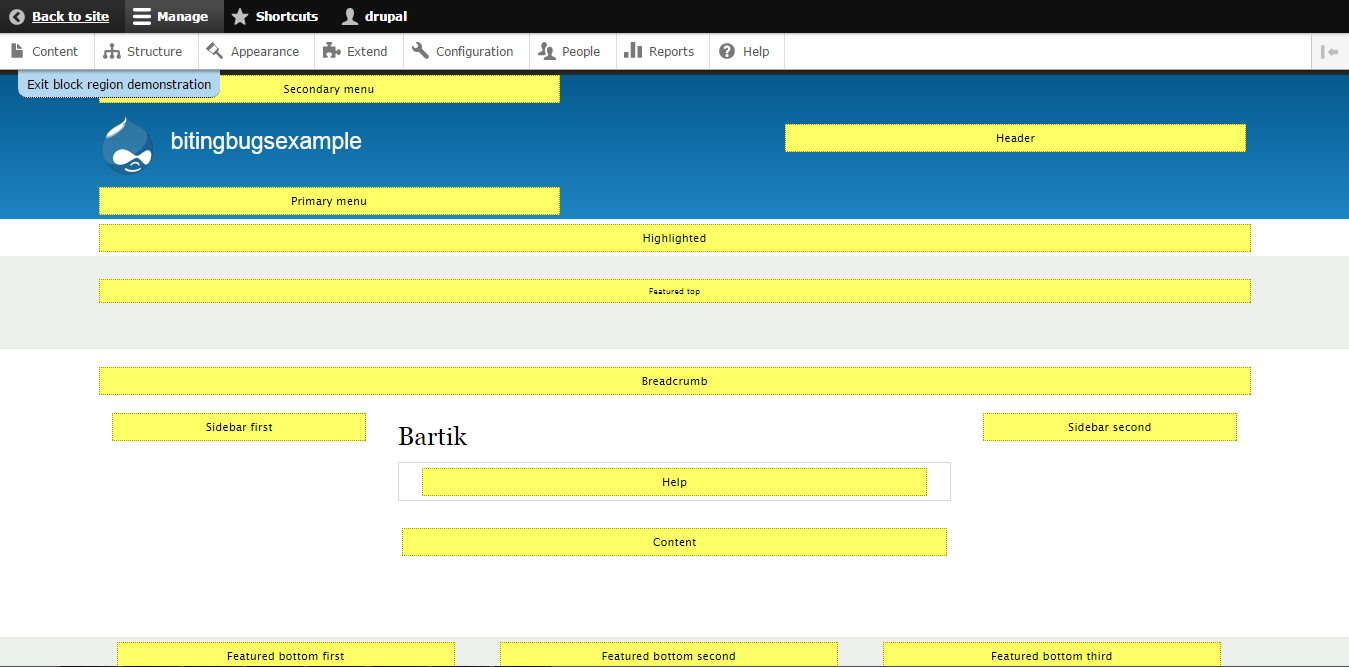
\includegraphics[width=\textwidth]{chapter4/region_demo}
  		\caption{Bartik regions}
  		\label{fig:region_demo}
  	\end{figure} 
  	
  	
  	\item[Comment types] The comment types page allows you to create and manage different comment types. When you add content to your site you can allow people to comment on the new content. The comment type defines the fields that the commenter has to fill out when he's writing his comment. The default comment type has only one field: the comment body. We could, for example, create a new comment type which includes a field for the name and age of the commenter. 
  	
  	\item[Contact form] The Personal contact form is the form for site visitors to contact registered users; the name and recipients of this form cannot be edited. Other forms listed here are your configured site-wide contact forms, which site visitors can use to send mail to a centralized email address or addresses. You can edit the name and recipients of site-wide forms by choosing the Edit operation. You can also configure the fields and display of both personal and site-wide forms.
  	
  	\item[Content types] The content types page is very important. The content types define which kind of information your CMS will manage. A content type has different fields. These fields define the information that is stored in the content type. 
  	By default Drupal has two content types: Article and Basic page (Figure \ref{fig:content_types});
  	
  	\begin{figure}[H]
  		\centering
  		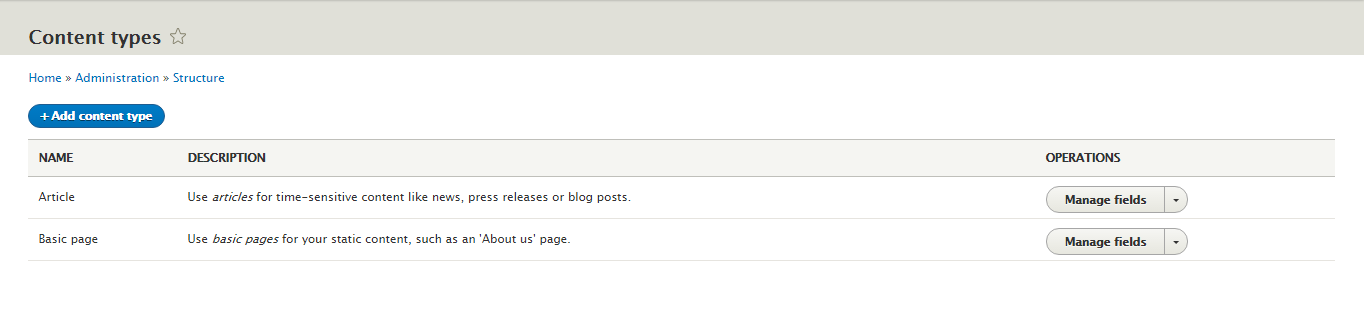
\includegraphics[width=\textwidth]{chapter4/content_types}
  		\caption{Default content types}
  		\label{fig:content_types}
  	\end{figure} 
  	
  	When you click the \textbf{Manage fields} button on the right you can see what kind of information is stored in this content type. (Figure \ref{fig:content_type_fields}). As you can see, the Article content type has four fields: Body, Comments, Image and Tags. 
  	
  	\begin{figure}[H]
  		\centering
  		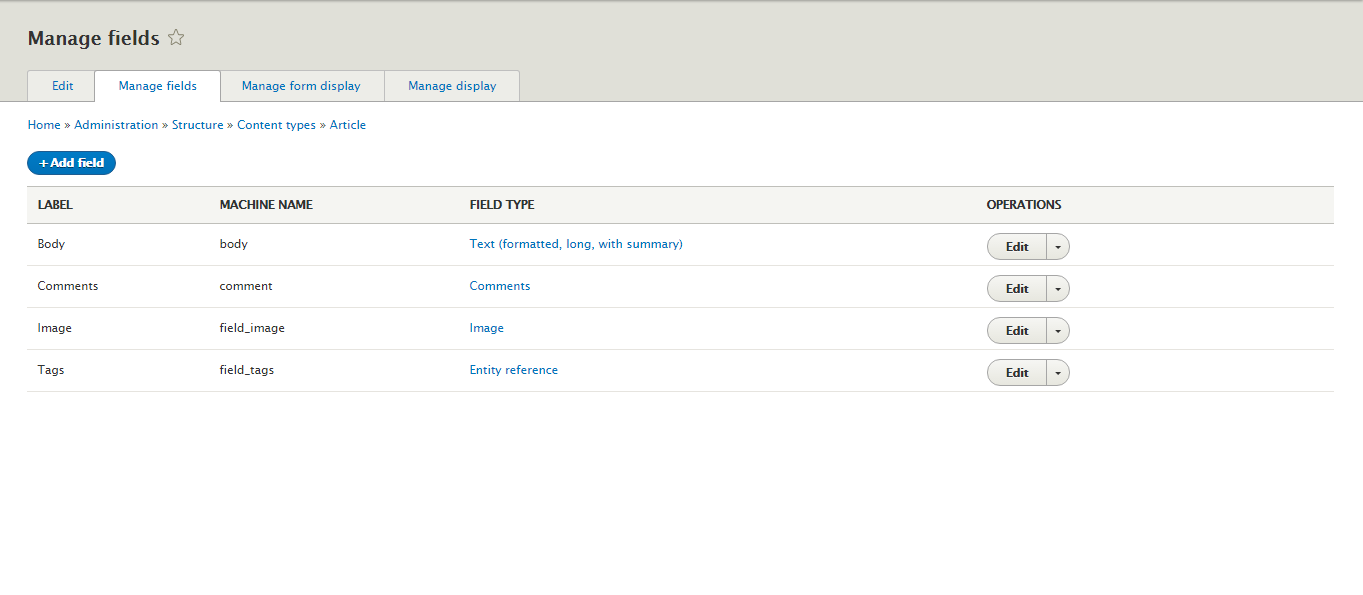
\includegraphics[width=\textwidth]{chapter4/content_type_fields}
  		\caption{Article content type fields}
  		\label{fig:content_type_fields}
  	\end{figure} 
  	
  	Next to the \textbf{Manage fields} menu item tab you have the \textbf{Manage form display} and \textbf{Manage display} tabs. These allow you to edit which fields are displayed when an element is created/edited or viewed.
  	
  	\item[Display modes] Display modes define different ways in which information is displayed. There are two types of display modes: form modes and view modes. Form modes are used when the content is created or edited, view modes when the content is viewed. 
  	When you go to \textbf{Display modes} $\rightarrow$ \textbf{View modes} (Figure \ref{fig:viewmodes}) you will see the different ways in which a content type can be displayed. 
  	
  		\begin{figure}[H]
  			\centering
  			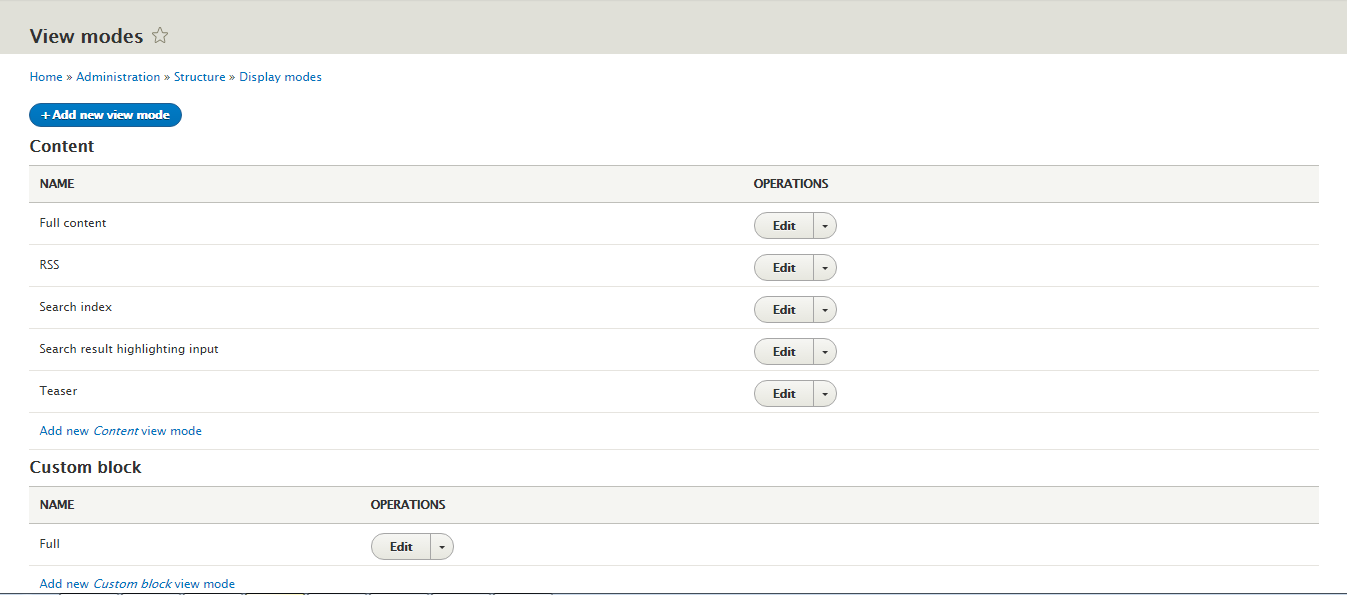
\includegraphics[width=\textwidth]{chapter4/viewmodes}
  			\caption{Default view modes}
  			\label{fig:viewmodes}
  		\end{figure}
  		
  	When you go to \textbf{Structure $\rightarrow$ Content types $\rightarrow$ Article $\rightarrow$ Manage display} you will see the following page:
  	
  	 \begin{figure}[H]
  	 	\centering
  	 	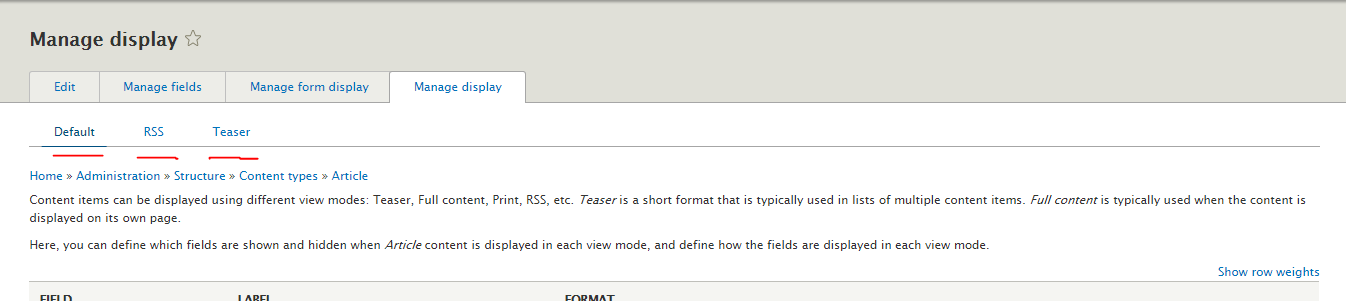
\includegraphics[width=\textwidth]{chapter4/display_types}
  	 	\caption{Display modes}
  	 	\label{fig:display_types}
  	 \end{figure}
  	 
  	 There you see the different display modes that you can use for your Article content type. At the bottom of the page you can enable other display modes in the custom display settings dropdown (Figure \ref{fig:custom_display_settings_dropdown}).
  	
  
  	\begin{figure}[H]
  		\centering
  		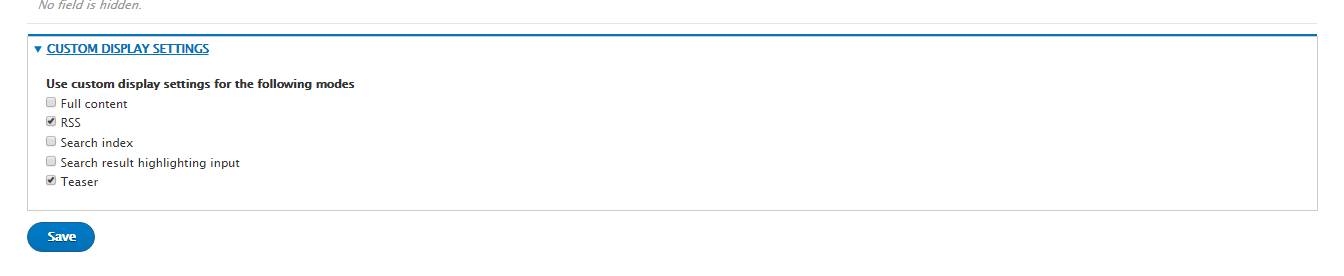
\includegraphics[width=\textwidth]{chapter4/custom_display_settings_dropdown}
  		\caption{Custom display settings}
  		\label{fig:custom_display_settings_dropdown}
  	\end{figure}
  	
  	\item[Menus] Menus are easy, they define a menu with different menu items. Each menu has a corresponding block that is managed on the Block layout page.
  	
  	\item[Taxonomy] A taxonomy defines lists of terms, these terms can be associated with the content. A list of terms is called a vocabulary. For example: if we have a site with news articles about sports we could add a tag to each article to tell what the article is about. These tags can be defined in a vocabulary. 
  	
  	\item[Views] A view enables you to create a display based on different content types. This course has a whole chapter dedicated to Drupal Views so we won't go into details here.
  	
  \end{description}
  
  \section{Bitingbugs example}
  
  In the following sections we will review the content of this chapter by applying it to an example website. In the previous chapter we created the bitingbugs example website through the Acquia Dev Desktop. In this and the following chapters we will keep adding features to this site. Our goal is to create a webstore for selling edible insects. The site will also provide a database with recipes so people know how to cook with the insects.
  
  \subsection{Change the site title and logo}
  
  To make our site a little bit prettier we will change the logo and title. To change the site title go to \textbf{Configuration $\rightarrow$ Site information}. There change the site name to \textbf{Biting Bugs} (Figure \ref{fig:bitingbugs_change_title}).
  
  \begin{figure}[H]
  	\centering
  	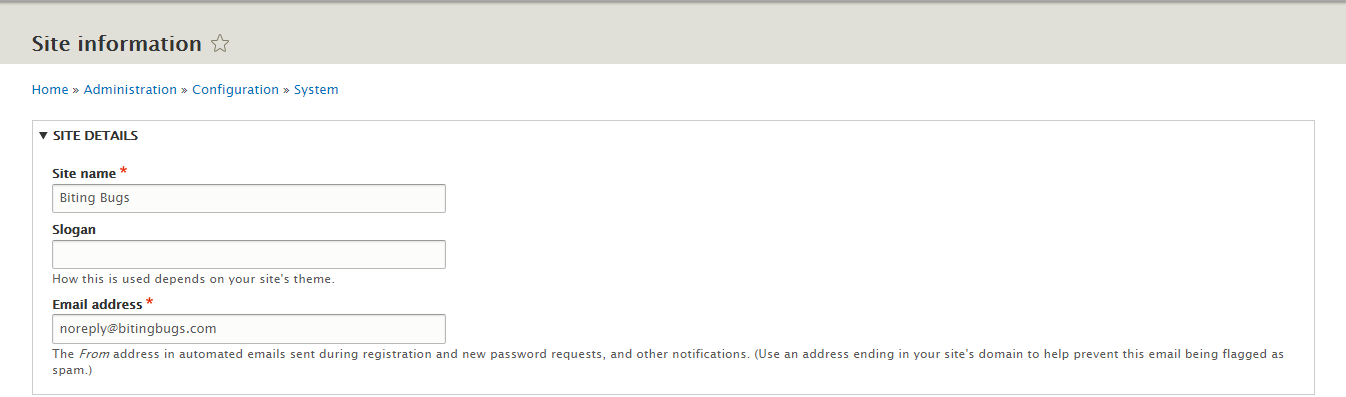
\includegraphics[width=\textwidth]{chapter4/bitingbugs_change_title}
  	\caption{Changing the site title}
  	\label{fig:bitingbugs_change_title}
  \end{figure}
  
  The logo is part of the Drupal theme you are using. To change the logo go to: \textbf{Appearance $\rightarrow$ Settings $\rightarrow$ Logo image settings}. Uncheck \textbf{Use the default logo supplied by the theme} and upload the file \url{bitingbugs_logo_transp_white_right_small.png} (Available in the course files zip). Click \textbf{Save configuration}.
  
  
  
  \begin{figure}[H]
  	\centering
  	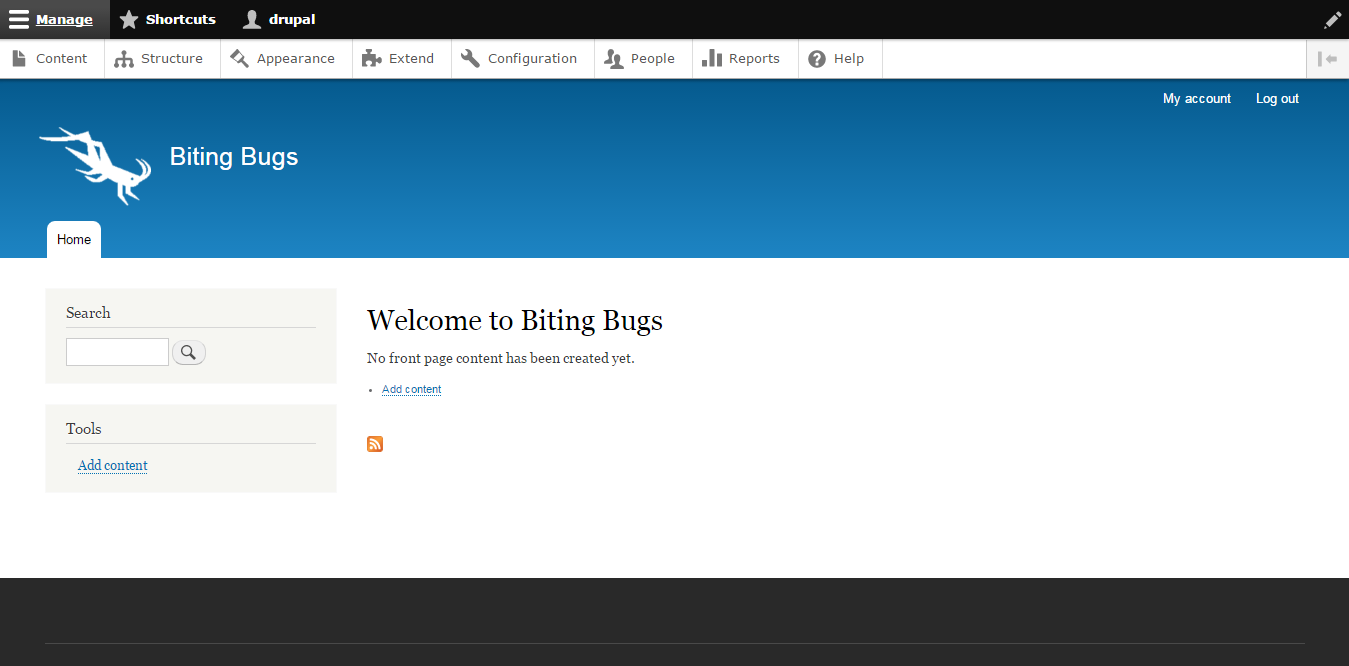
\includegraphics[width=\textwidth]{chapter4/bitingbugs_logo_and_title_changed}
  	\caption{Changed logo and title}
  	\label{fig:bitingbugs_logo_and_title_changed}
  \end{figure}
  
  \subsection{Removing the Search and Tools block}
  
  On the right side of the page we have the \textbf{Search} and \textbf{Tools} block. We don't need them for now so you can remove them by going to \textbf{Structure $\rightarrow$ Block layout} and moving them from the \textbf{Sitebar first} to the \textbf{None} region (Figure \ref{fig:bitingbugs_remove_search_block}). Click \textbf{Save blocks}.
  
  \begin{figure}[H]
  	\centering
  	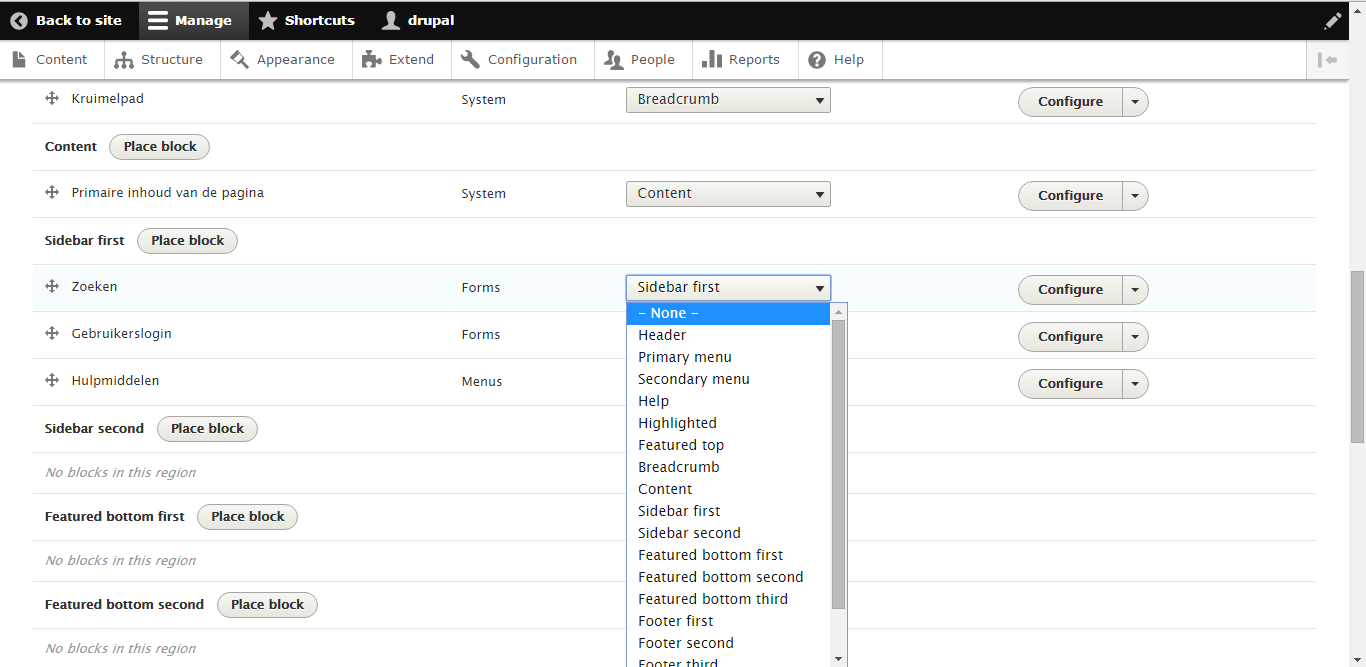
\includegraphics[width=\textwidth]{chapter4/bitingbugs_remove_search_block}
  	\caption{Remove a block from a region}
  	\label{fig:bitingbugs_remove_search_block}
  \end{figure}
  
  \subsection{Adding a Taxonomy}
  
  To categorise the recipes on our site we will add a taxonomy. This taxonomy will contain different types of dishes. Go to \textbf{Structure $\rightarrow$ Taxonomy $\rightarrow$ Add vocabulary}. Use the following settings: 
  
  \begin{description}
  	\item[Name:] Dish types
  	\item[Description:] Describes the type of dish we will add.
  	\item[Vocabulary language] English
  	\item[Default language] Site's default language (English)
  \end{description}
  
  \begin{figure}[H]
  	\centering
  	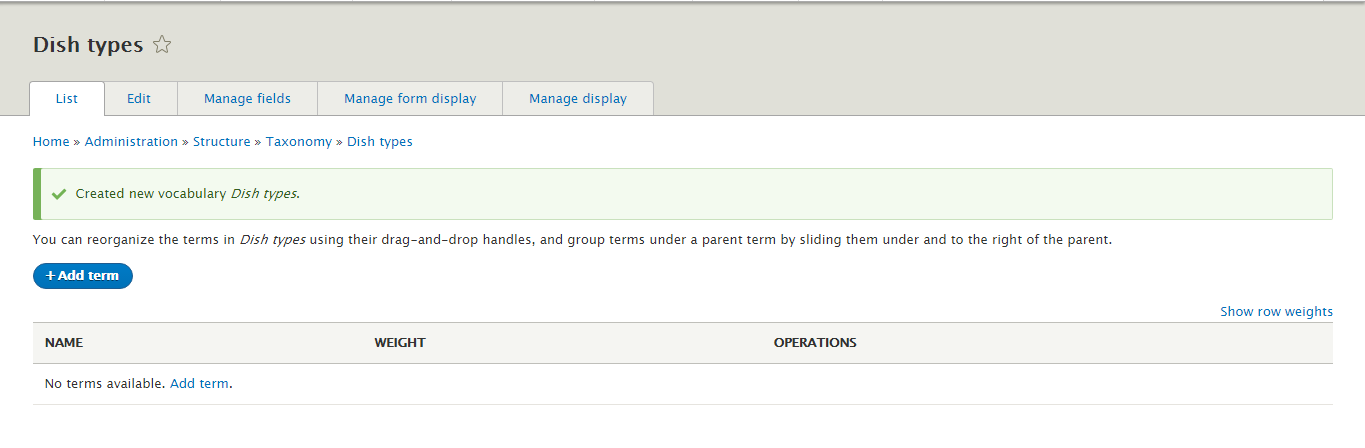
\includegraphics[width=\textwidth]{chapter4/bitingbugs_add_dish_types}
  	\caption{Adding a vocabulary terms}
  	\label{fig:bitingbugs_add_dish_types}
  \end{figure}
  
  Click \textbf{Save}. In Figure \ref{fig:bitingbugs_add_dish_types} you can see the empty vocabulary. Next we will add some terms to the vocabulary. Click the \textbf{Add term} button and add the following terms:
  
  \begin{itemize}
  	\item candy
  	\item curry
  	\item dessert
  	\item pasta
  	\item salad
  	\item sandwiches 
  	\item sauces
  	\item vegetarian
  	\item vegan
  \end{itemize}
  
  
    \begin{figure}[H]
    	\centering
    	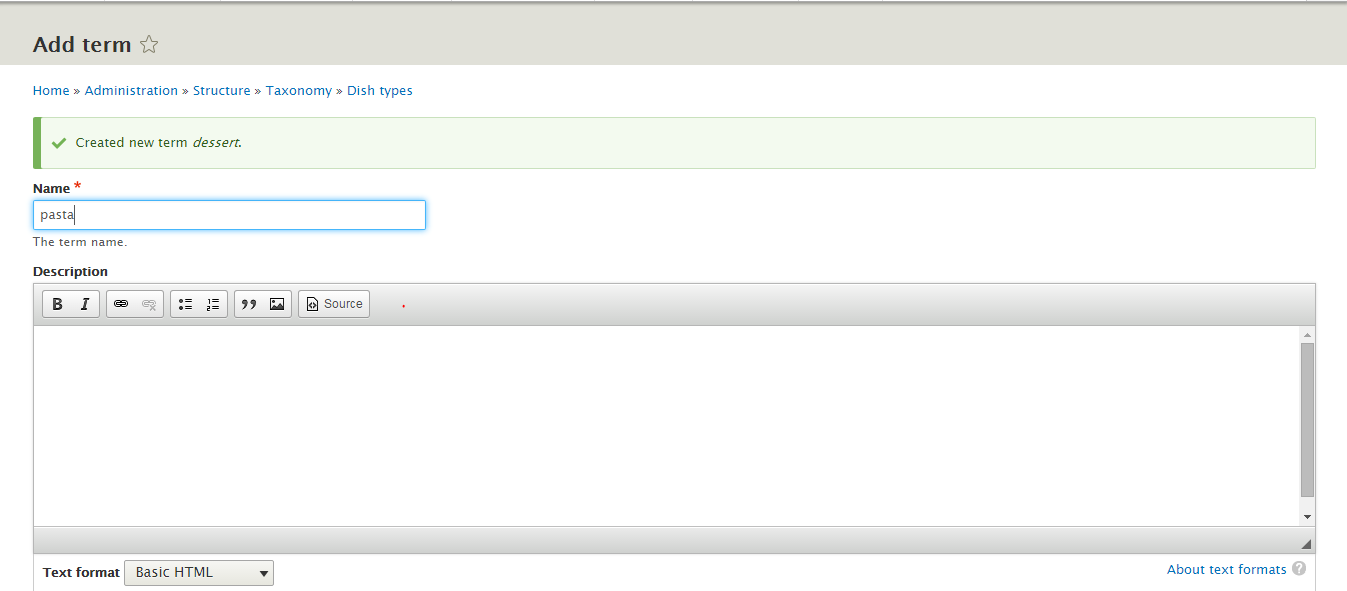
\includegraphics[width=\textwidth]{chapter4/bitingbugs_add_vocabulary_terms}
    	\caption{Adding a vocabulary term}
    	\label{fig:bitingbugs_add_vocabulary_terms}
    \end{figure}
    
    To see an overview of the terms you have added go to \textbf{Structure $\rightarrow$ Taxonomy} and click the \textbf{List items} button next to your vocabulary. (Figure \ref{fig:bitingbugs_dish_types})
    
    \begin{figure}[H]
    	\centering
    	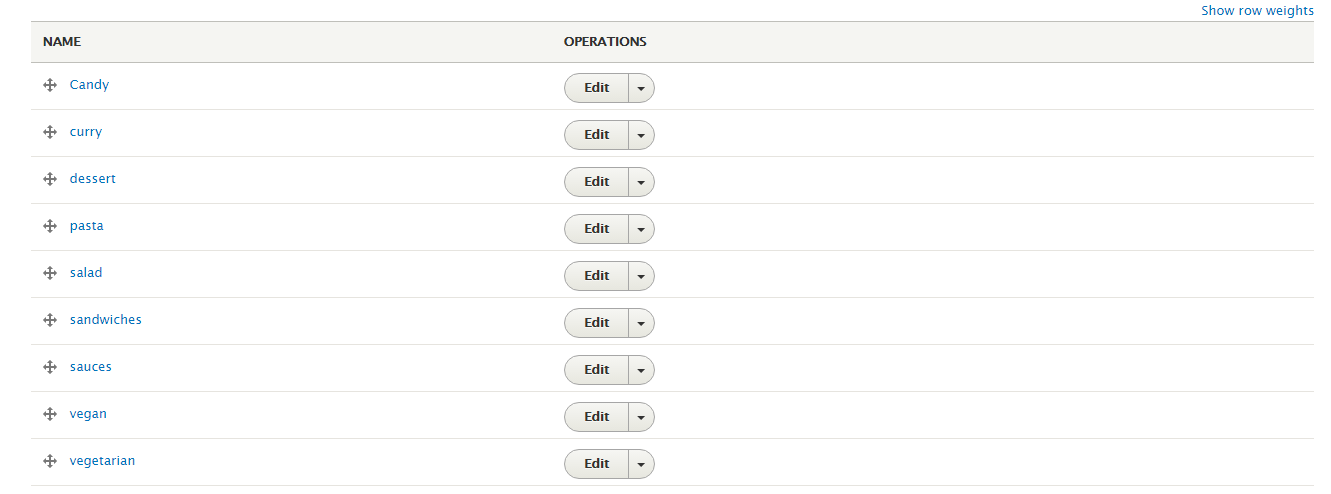
\includegraphics[width=\textwidth]{chapter4/bitingbugs_dish_types}
    	\caption{Vocabulary terms}
    	\label{fig:bitingbugs_dish_types}
    \end{figure}
    
    \subsection{Adding the \textbf{Recipe} content type}
    
    Since we are going to store recipes in our CMS we will need to add the \textbf{Recipe} content type. Go to: \textbf{Structure $\rightarrow$ Content types $\rightarrow$ Add content type}. Give it the following properties:
    
    \begin{description}
    	\item[Name:] Recipe 
    	\item[Description] A recipe for cooking bugs!
    \end{description}
    
    At the bottom of the page you can see some settings for this content type. Explore the settings, the names are very descriptive so most of them should be clear without further explanation. These are general settings that apply to all instances of this content type. You are able to change these for each instance individually when you create them.
    
    Click \textbf{Save and manage fields}.
    
    
    \begin{figure}[H]
    	\centering
    	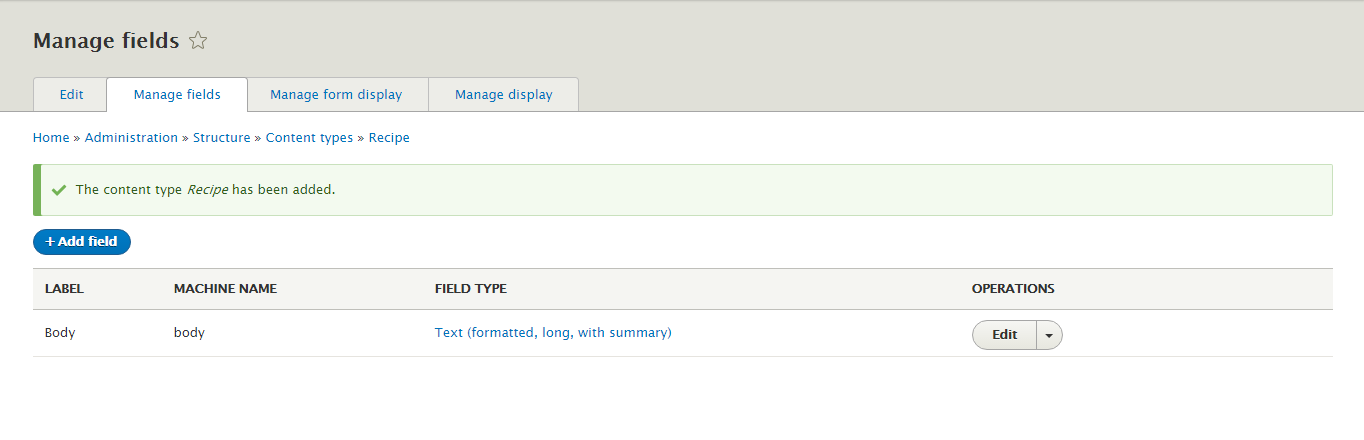
\includegraphics[width=\textwidth]{chapter4/bitingbugs_manage_recipe_fields}
    	\caption{Manage recipe fields}
    	\label{fig:bitingbugs_manage_recipe_fields}
    \end{figure}
    
    Add the following fields to the \textbf{Recipe} content type:
    
    \begin{description}
    	\item[Name] (Text/plain, Maximum length = 255, number of values = 1) 
    	\item[Ingredients] (Text/plain, Maximum length = 255, number of values = unlimited)
    	\item[Body] (already there)
    	\item[Plate image] (Image, number of values = 1)
    	\item[Estimated time] (Number(decimal), number of values = 1, Help text = Estimated time to cook the recipe in minutes).
    	\item[Type] (Taxonomy term, number of values = unlimited, reference method = default, Vocabularies: Dish types, Create referenced entities if they don't already exist).
    \end{description}
    
    In figure \ref{fig:bitingbugs_recipe_fields} you can see an overview of the fields.
    
    \begin{figure}[H]
    	\centering
    	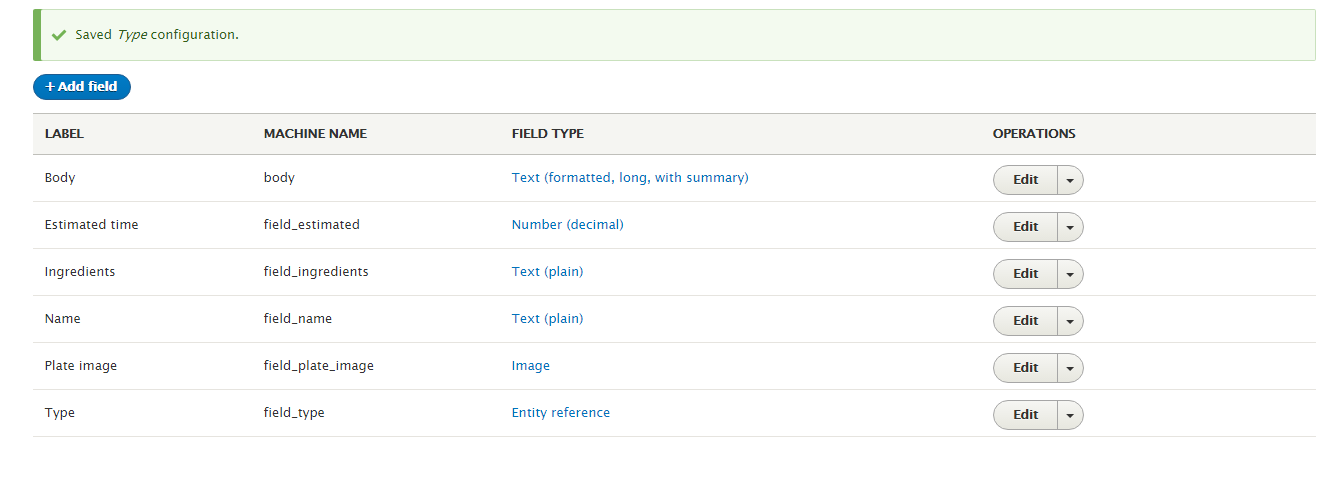
\includegraphics[width=\textwidth]{chapter4/bitingbugs_recipe_fields}
    	\caption{Recipe fields}
    	\label{fig:bitingbugs_recipe_fields}
    \end{figure}
  
  \section{review exercises}
  
  \begin{enumerate}
  	\item Log in to your \textbf{exploringdrupal8} site (created in the previous chapter). Add the search block to the \textbf{sidebar second} region and disable the \textbf{powered by Drupal} block.
  	
  	
  	\item Add a comment type \textbf{Answer} to your \textbf{exploringdrupal8} site. We will use the comment type to allow users to answer a question. The comment type has two fields: answer (a number between 0 and 100000) and motivation (a textual explanation describing how they got the answer).
  	
  	\item Add a new content type \textbf{recipe} to your \textbf{exploringdrupal8} site. The new content type has the following fields: Title, PlateImage (Image), ingredients (list), description. Make sure the teaser only displays the Title and Image fields.
  	
  	\item Add a vocabulary \textbf{Food types} to your \textbf{exploringdrupal8} site. Add the following terms to the vocabulary: Indian, Chinese, vegetarian, vegan. 
  	
  	
  \end{enumerate}